\documentclass{article}

% if you need to pass options to natbib, use, e.g.:
% \PassOptionsToPackage{numbers, compress}{natbib}
% before loading nips_2016
%
% to avoid loading the natbib package, add option nonatbib:
% \usepackage[nonatbib]{nips_2016}

% \usepackage{nips_2016}
\usepackage[final]{nips_2016}
\usepackage{graphicx}
\usepackage{caption}
\usepackage{subcaption}
\usepackage{placeins}
\usepackage{float}

% to compile a camera-ready version, add the [final] option, e.g.:
% \usepackage[final]{nips_2016}

\usepackage[utf8]{inputenc} % allow utf-8 input
\usepackage[T1]{fontenc}    % use 8-bit T1 fonts
\usepackage{hyperref}       % hyperlinks
\usepackage{url}            % simple URL typesetting
\usepackage{booktabs}       % professional-quality tables
\usepackage{amsfonts}       % blackboard math symbols
\usepackage{nicefrac}       % compact symbols for 1/2, etc.
\usepackage{microtype}      % microtypography

\title{Computational Analyses Supporting Diverse Synaptic Clusters In Mouse Cortex}

% The \author macro works with any number of authors. There are two
% commands used to separate the names and addresses of multiple
% authors: \And and \AND.
%
% Using \And between authors leaves it to LaTeX to determine where to
% break the lines. Using \AND forces a line break at that point. So,
% if LaTeX puts 3 of 4 authors names on the first line, and the last
% on the second line, try using \AND instead of \And before the third
% author name.

\author{
  Adam Li \\
  Department of Biomedical Engineering\\
  Johns Hopkins University\\
  Baltimore, MD 21210 \\
  \texttt{ali39@jhu.edu} \\
  \And
  Tyler Tomita \\
  Department of Biomedical Engineering\\
  Johns Hopkins University\\
  Baltimore, MD 21210 \\
  \texttt{tmtomita87@gmail.com} \\
  \And
  Joshua Vogelstein, PhD \\
  Department of Biomedical Engineering\\
  Johns Hopkins University\\
  Baltimore, MD 21210 \\
  \texttt{jovo@jhu.edu} \\
}

\begin{document}

\maketitle

\begin{abstract}
  Currently, very little is understood about the synaptic connections within our brain. Our original belief is that there are only two types of synapses: excitatory and inhibitory. However, it is now known that there is a much more diverse synapse population. We want to characterize these different subpopulations by protein expressions. Here we present an analysis of protein expressions under Array Tomography at synaptic locations. Our initial results show evidence pointing towards a richer set of sub-synaptic clusters then just excitatory and inhibitory. 
\end{abstract}

\section{Introduction}

Many hundreds of distinct proteins are involved in the development of synapses and mechanisms in synaptic signaling. Although complex, this molecular architecture can enable a better characterization of synaptic populations and subgroups based on protein clustering. We are aware of excitatory and inhibitory synapses, but it is now known there is a much more diverse set of subpopulations \cite{Wheeler2015,Usoskin2014a}.

Differences in protein expression patterns at individual synapses could constitute a key to understanding synaptic diversity. The dataset analyzed in this paper was produced by Weiler, et al. using array tomography (ATomo) to image the synaptic molecular architecture of neighboring whisker-associated columns of the mouse somatosensory cortex \cite{Weiler2014}. ATomo is well suited to proteomic mapping of synaptic circuits because ultrathin sectionining of resin-embedded tissue samples enable immunohistochemical multiplexing and high-resolution imaging of millions of synapses \cite{Micheva2007}. These images were then reconstructed into precisely aligned image volumes, with data on millions of synapses in the image volume.

It is difficult to sift through millions of synaptic locations and determine subgroups by eye. With the development of increasing computational power and machine learning techniques, it is becoming easier to analyze large datasets and glean information on trends and clusters. Here, we employ a data driven approach to computationally analyze the synapse population of this dataset to glean insights into synaptic clusters. 

\section{Methods}
\label{methods}

\subsection{Data}
Data was gathered from the Array Tomography section of http://openconnecto.me/, the OpenConnectome project. The data we received were two matrices that represented the features and the <x,y,z> image volume coordinate locations for each synapse location. Preprocessing was done to identify synapses based on the Synapsin expression levels in the ATomo pipeline, based on a set threshold \cite{Weiler2014}. The resulting feature matrix was a 1119299 x 96 matrix, with the rows representing a single synapse location and the columns representing 24 protein measurements of integrated brightness (f0), local brightness (f1), distance to center of mass (f2) and moment of inertia around synapse (f3). There were 24 different protein measurements done per f0-f3. The protein markers belong to one of seven functional groupings as outlined in Table ~\ref{fig:table1}. In addition to ATomo imaging data, each synapse (or row) has an estimated location in the image space represented by a matrix 1119299 x 3. They represent 3D pixel locations at the nm scale. 

\subsection{Preprocessing}
In our analysis, we began with an overall analysis of the four different metrics and then analyzed the metric we deemed most important separately afterwards. We implemented a pairwise correlation computation to look at correlations among features. Then we applied an arbitrary threshold of 0.6 to see which features correlated higher then the thresdhold. By analyzing only one metric among f0-f3, the feature matrix of interest is now 1119299 x 24. Since the scales of each protein channel measurement varied, we applied a log-normalization transformation, which meant scaling all columns to [0, 1] and then applying a log transformation.

We chose to focus on f0 (integrated brightness) because of its correlative measurements. We first checked the validity of the data. Since there were repeated measurements for the same protein, the measurements should all lie within a linear regression. We created a pairwise scatter plot for repeated Synapsin and VGlu1 measurements and looked at the linear regression to check for linearity and hence valid data measurements for f0.

Since we are looking for subclusters of synapse types, it would be biased to only have synapses heavily located in one region of the tissue volume. Therefore, we inspected whether or not there seemed to be a uniformly distributed sample of synapses throughout the tissue volume by plotting histograms along the <x,y,z> axis.

\subsection{Cluster Analysis and Principle Component Analysis}
Due to the size of our dataset, it was computationally infeasible to apply a regular KMeans unsupervised clustering algorithm to the dataset. Therefore, we used the MinibatchKMeans algorithm available in Python, which has been shown to achieve similar results in shorter computation time \cite{Sculley2010}. To determine optimal cluster number k, we implemented a Bayesian Information Criterion (BIC) analysis that scored the likelihood of the data within a cluster and the cost of number of clusters there were \cite{Fallis2013}. Once an optimal k was estimated, we performed the MinibatchKMeans clustering on the preprocessed feature matrix, and looked at the Euclidean distance between centroids of clusters. 

Although there are 24 different protein measurements, we sought to reduce the dimensionality of via principle component analysis (PCA) \cite{Wold1987}. Here we plotted scree plots to visualize the number of components needed to account for the variance in our data. 

\section{Results}
\label{results}

In the analysis of all metrics f0, f1, f2 and f3, we generated a pairwise correlation plot to determine correlations within our feature set. Figure ~\ref{fig:figure1} shows a pairwise correlation plot and a thresholded pairwise correlation plot. It seems that f0 highly correlates with itself, which is something we should expect since it is the same metric. We therefore, choose to first focuse on f0 (integrated brightness) for the remainder of our analyses. 

In our validation of integrated brightness measurement, we saw a linear trend in the pairwise scatter plot of both repeated protein measurements, Synapsin and VGlut1. This is what we expected to see since the ATomo should only produce a linear range of values. We then looked at the distribution of synapses throughout the image volume and see that it is looks distributed throughout the image volume without any visual clustering in one region over another.

Next we analyzed the BIC scores for different k using the MinibatchKMeans algorithm on the data. Since synapses were identified by the expression of Synapsin values, we took the synapses (rows in matrix) with top 25, 50 and 75\% of Synapsin value and also analyzed the BIC score to see if it was sensitive to our thresholding of a synapse. We found that all BIC plots produced a relative elbow around k=4, so we proceeded with clustering the entire dataset with k=4. In figure ~\ref{fig:figure4}, it shows the pairwise Euclidean distance plot between the different centroids used in KMeans of 4, where we see a maximum distance of 0.72 between cluster centroids and ~0.30 distance between cluster centroids on the off-diagonal. The diagonal are all 0 because it represents cluster centroids compared with itself. 

When we implemented a PCA on our 1119299 x 24 feature matrix, we found that only 5 principle components were needed to account for 90 percent of our variance in our data, while ~12 prinnciple components accounted for almost all the data variance. This means that any clustering based on variance of our data could be reduced down from 24 dimensions to 12, or even 5, if we only care about up to 90 percent of data variance. 

\section{Discussion}
\label{discussion}
We have shown an initial analysis of the protein expression data at synapses identified using ATomo. Overall, we have shown evidence that there are indeed more then just an excitatory and inhibitory clustering of synapses. We have seen that integrated brightness is highly correlative with itself relative to the other metrics involved (local brightness, distance to center of mass and moment of inertia around synapse). By focusing our analysis on integrated brightness, we saw that an approximate optimal number of clusters was 4.

When we tested that initial assumption by plotting pairwise distance plots of the centroids, we saw that they were relatively distanced against each other. In addition, when reducing the dimensionality of the protein channels, we saw that ~4, or 5 principle components accounted for 90\% of the data variance. If the synapse populations are characterized by integrated brightness variance in protein expression, then this would also support our inclination that our dataset captures at least 4 unique clusters. Reducing the dimensions down to 12 would only leave <1\% of variance unaccounted for, while increasing the interpretability of the data.

In upcoming work, we would like to 1. validate our clustering scheme and how the distribution of protein expression looks within each cluster and 2. test different subclustering algorithms. By validating our clustering scheme, we can determine if there is a clustering of just excitatory and inhibitory synapses first. This would mean most of the proteins expressed in excitatory are in one cluster, and vice versa. We can also try various subspace clustering algorithms that utilize l1 and l2 regularizations for sparsity and smoothness \cite{You}. This showed a computationally efficient way of subspace clustering using elastic net and can be easily implemented.


\newpage
\section{Citations, figures, tables, references}
\label{others}

\FloatBarrier
\subsection{Figures}
% Correlation Plot
\begin{figure}[!htb]
  \centering 
  \begin{subfigure}[b]{0.49\textwidth}
    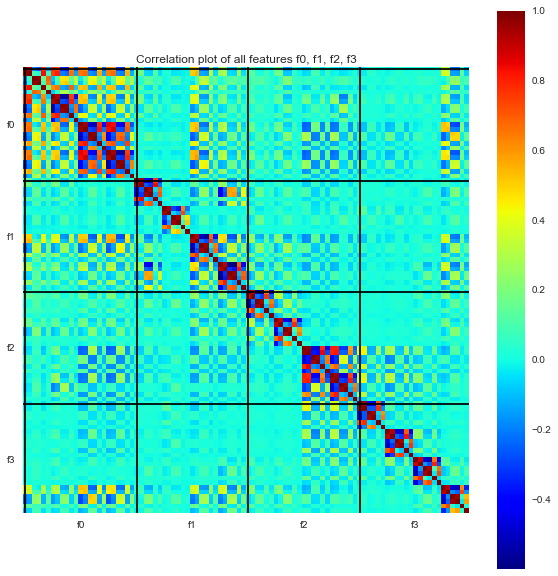
\includegraphics[width=70mm]{figures/corrplot.png}
    \caption{}
    \label{fig:figure1a}
  \end{subfigure}
  \begin{subfigure}[b]{0.49\textwidth}
    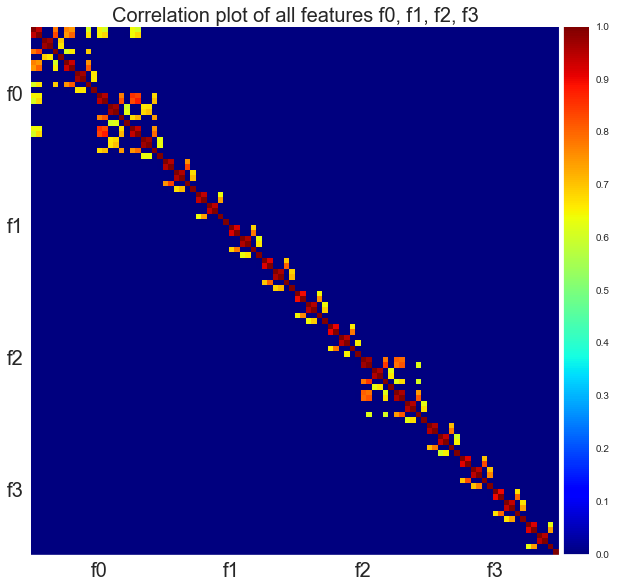
\includegraphics[width=70mm]{figures/thresholdcorrplot.png}
    \caption{}
    \label{fig:figure1b}
  \end{subfigure}
  \caption{Pairwise correlation plots of the entire feature set, with (a) being the correlation plot without a threshold, and (b) having a threshold of 0.6 applied. All correlations less than or equal to 0.6 were set to 0.}
  \label{fig:figure1}
\end{figure}

% f0 Data Check
\begin{figure}
  \centering 
  \begin{subfigure}{\textwidth}
    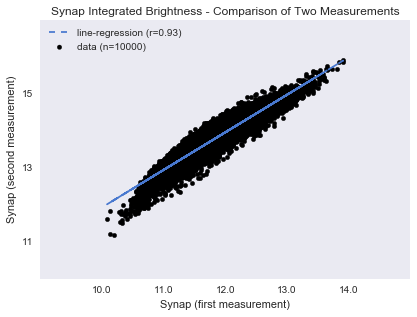
\includegraphics[width=\textwidth]{figures/data_check01.png}
    \caption{}
    \label{fig:figure2a}
  \end{subfigure}
  \begin{subfigure}{\textwidth}
    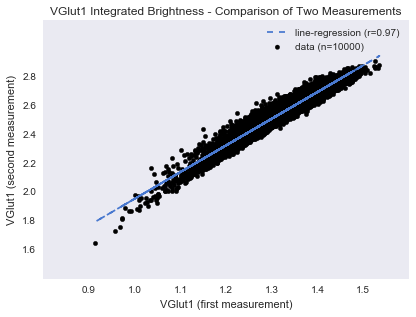
\includegraphics[width=\textwidth]{figures/data_check02.png}
    \caption{}
    \label{fig:figure2b}
  \end{subfigure}

  \caption{Pairwise scatter plots of the repeated measurements of Synapsin (a) and VGlut1 (b), showing the integrated brightness.}
  \label{fig:figure2}
\end{figure}

% f0 Location Data Check
\begin{figure}
  \centering 
  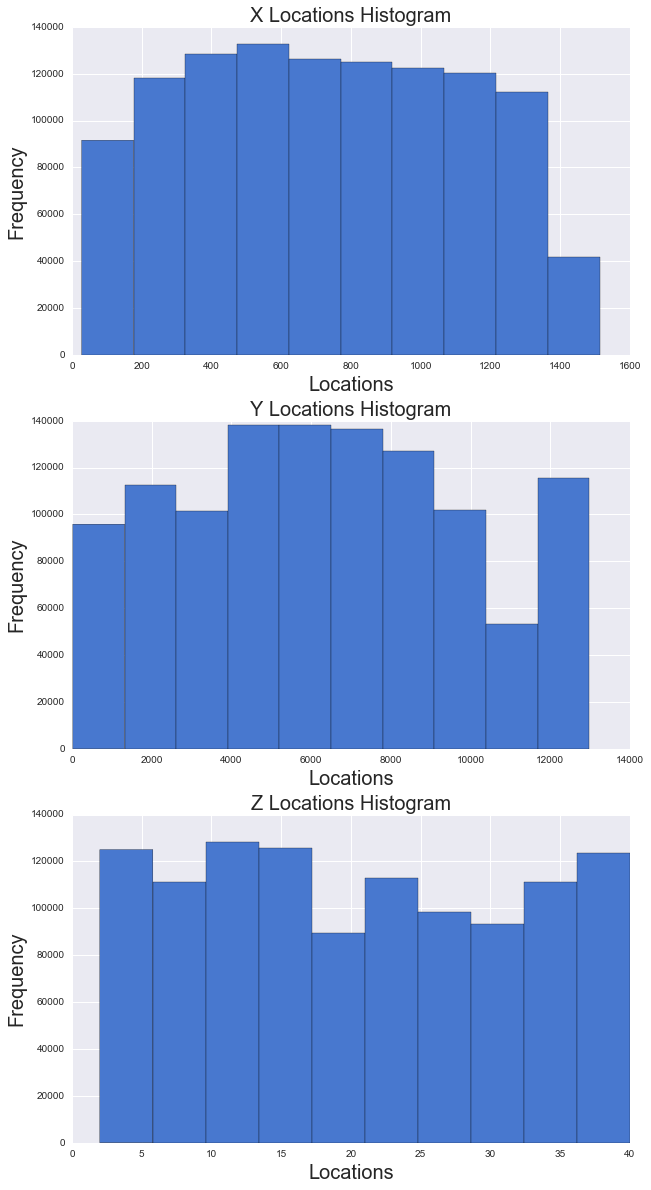
\includegraphics[scale=0.5]{figures/locationshist.png}
  \caption{Histogram plots showing the distribution of synapses at locations throughout the image volume.}
  \label{fig:figure3}
\end{figure}

% Figure lognormalized BIC plot
\newpage
\begin{figure}
  \centering
  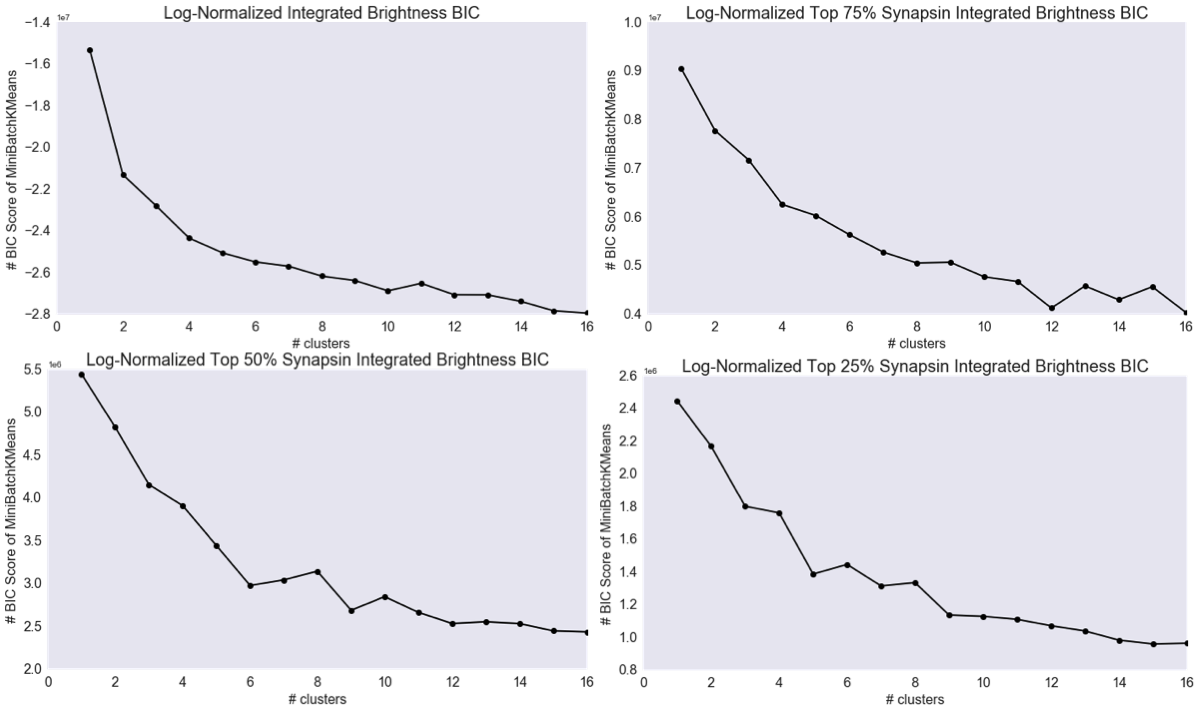
\includegraphics[width=\textwidth]{figures/exploratory/logbicplot.png}
  \caption{Figure (a) showing a BIC plot generated using MinibatchKMeans with a k={1,..,16} on the integrated brightness values. (b,c,d) show the BIC plots with the bottom 25, 50, and 75 percent Synapsin values filtered out respectively.}
  \label{fig:figure4}
\end{figure}

% Figure of KMeans=4
\begin{figure}
  \centering
  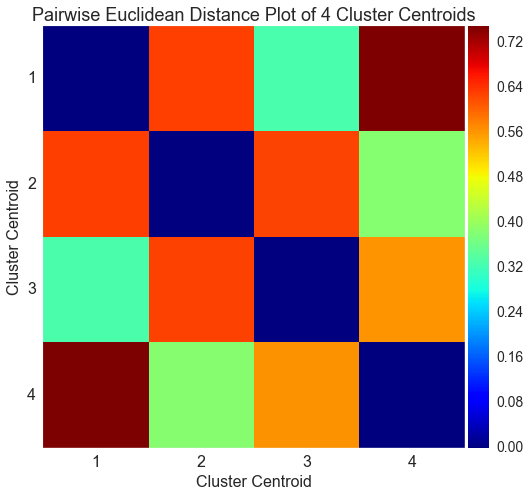
\includegraphics[scale=0.5]{figures/cluster4pairwisedistance.png}
  \caption{KMeans clustering with k=4. Along the diagonal all pairwise distances are equal to 0.0, while the off diagonals show relative euclidean distance. All off diagonals are relatively spaced away from each other with a minimum euclidean distance of ~0.3.}
  \label{fig:figure5}
\end{figure}

% Figure Scree Plots
\begin{figure}
  \centering
  \begin{subfigure}{0.49\textwidth}
    \label{fig:figure6a}
    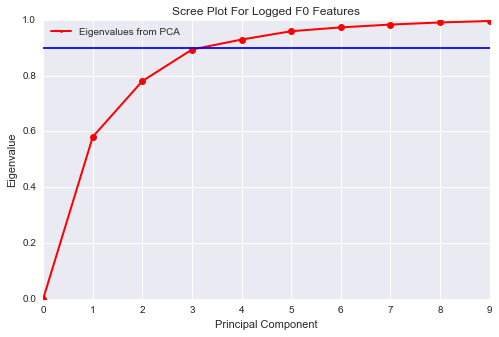
\includegraphics[width=75mm]{figures/exploratory/f0_lognormalized_screeplot.png}
    \caption{}
  \end{subfigure}
  \begin{subfigure}{0.49\textwidth}
    \label{fig:figure6b}
    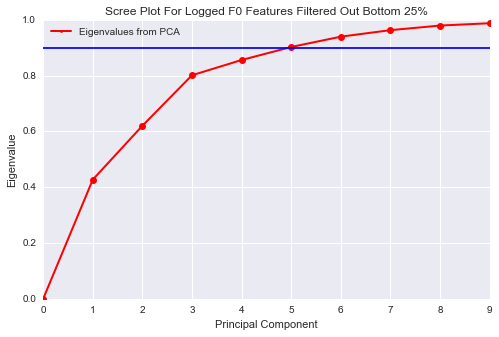
\includegraphics[width=75mm]{figures/exploratory/f0_lognormalized_bottom25_screeplot.png}
    \caption{}
  \end{subfigure}
  \begin{subfigure}{0.49\textwidth}
    \label{fig:figure6c}
    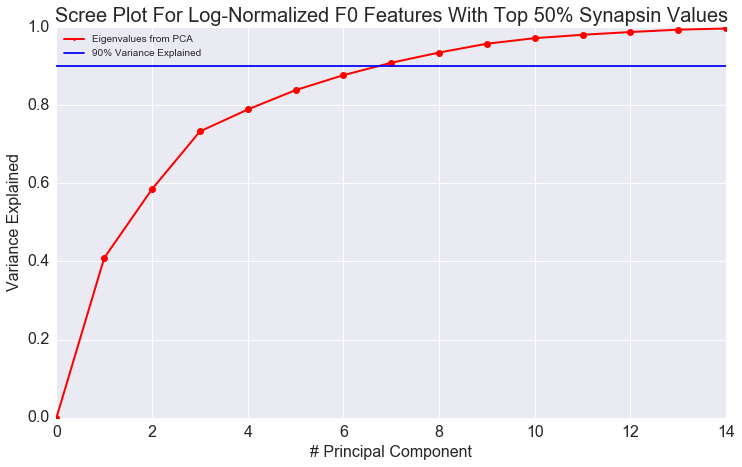
\includegraphics[width=75mm]{figures/exploratory/f0_lognormalized_bottom50_screeplot.png}
    \caption{}
  \end{subfigure}
  \begin{subfigure}{0.49\textwidth}
    \label{fig:figure6d}
    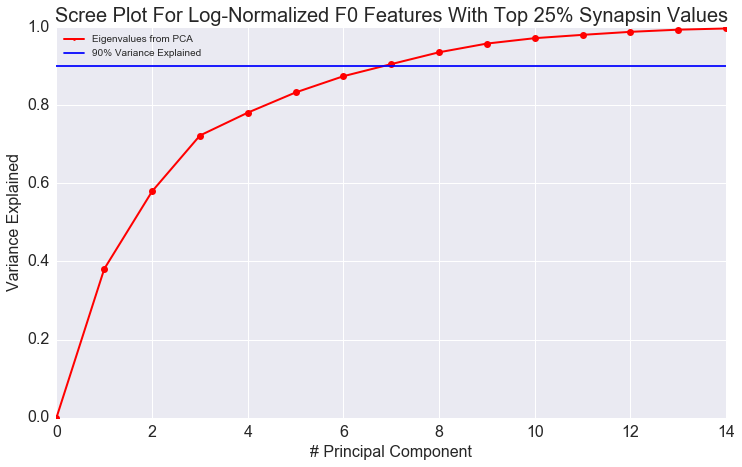
\includegraphics[width=75mm]{figures/exploratory/f0_lognormalized_bottom75_screeplot.png}
    \caption{}
  \end{subfigure}
  \caption{Figure (a) showing a scree plot on the entire lognormalized dataset on the integrated brightness values. (b,c,d) show the scree plots with the bottom 25, 50, and 75 percent Synapsin values filtered out respectively. The solid line represents 90\% variance.}
  \label{fig:figure6}
\end{figure}

\FloatBarrier
\subsection{Tables}

% Table of Protein Groups
\begin{table}[H]
  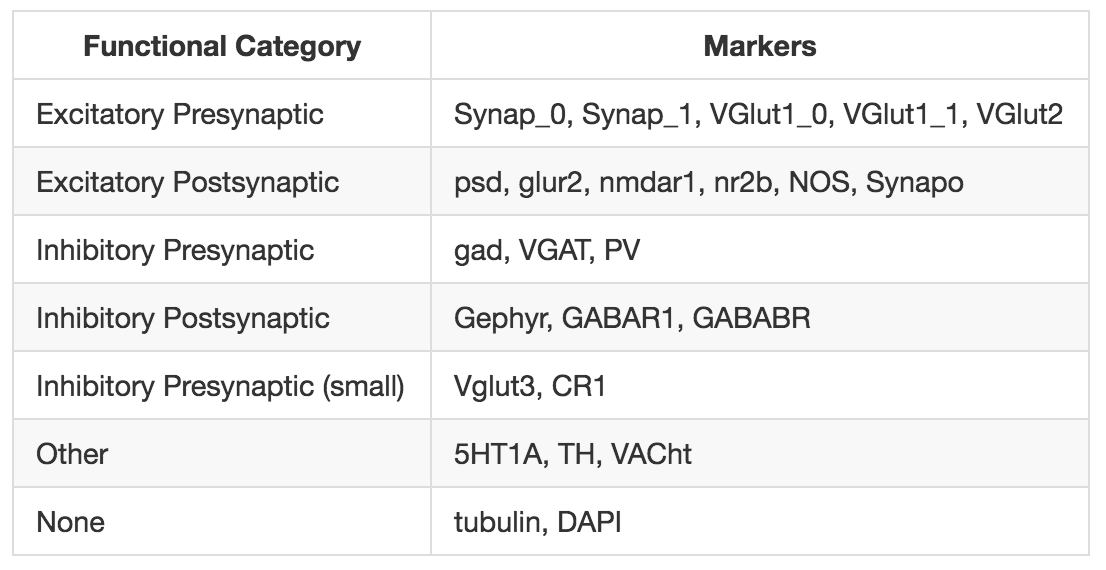
\includegraphics[width=\linewidth]{figures/table1.png}
  \caption{Table 1: Table showing the data collectors providing domain knowledge regarding groupings of the 24 protein markers. Each marker belongs to one of seven functional groupings.}
  \label{fig:table1}
\end{table}

\FloatBarrier
\subsection{Equations}

Bayesian Information Criterion Variables:
\begin{description}
\item[$\bullet$] N: total number of data points
\item[$\bullet$] m: total number of clusters
\item[$\bullet$] $n_i$: size of each cluster i
\item[$\bullet$] d: total number of features per data point
\item[$\bullet$] D: represents the variable for clusters
\end{description}

The BIC score is formally defined as 
BIC($\phi$) = $l\widehat{}_{\phi}(D) - \frac{p_{\phi}}{2}*log(N)$

With:
\[l\widehat{}_{\phi}(D) = \sum_i (n_i * log(n_i)) - Nlog(N) - \sum_i\frac{(n_i d)}{2} * log(2\pi\sigma{}\widehat{}^2)
\]
\[
\frac{p_{\phi}}{2}*log(N) = \frac{d}{2}(N-m) - 0.5m(d+1)log(N)
\]
\[
\sigma{}\widehat{}^2 = \frac{1}{N-m} \sum{||x{}_i - \mu{}_i||}^2
\]

% references
\newpage
\small
{
  \bibliography{/Users/adam2392/Documents/Bibtex/Synapse_Diversity.bib}
  \bibliographystyle{plain}
}

\end{document}
